% !TEX root =  ../report.tex

\section{Research}
\label{s:research}

\subsection{NVidia CUDA Programming Model}
Since this project will require the automatic generation of GPU code source files from sequential code, it is important to introduce the NVidia hardware, and the C Application Programming Interface (API) which will be utilised. NVidida's Compute Unified Device Architecture (CUDA) is used to program their GPUs, which is a proprietary language. Relevant information for this project from the \textit{NVidia CUDA C Programming Guide} \cite{guide} has been summarised below, and it will continue to be used for reference throughout this report.

\subsubsection{Hardware}
The GPU is a computer component that exisits alongside the CPU, and communicates on the PCI express bus. The CPU is able to pass workloads over to the GPU for it to execute, particularly compute-heavy workloads which would bottleneck the CPU. As can be seen in Figure \ref{fig:pci}, the GPU has its own onboard memory, and cannot access the computer's RAM, so any data that the GPU will process must be copied across the PCIe bus and stored in the GPU's local memory, at the expense of time.

\begin{figure}[h!]
  \centering
  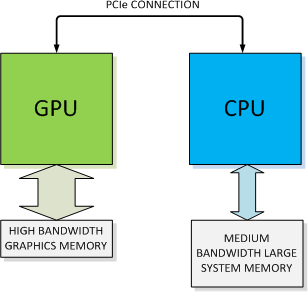
\includegraphics[width=0.5\textwidth]{pci}
  \caption{\label{fig:pci} CPU - GPU communication. Diagram from \cite{nvlink}}
\end{figure}

\par
Figure \ref{fig:arch} constrasts the design of a traditional CPU to that of a GPU, where area of a component corresponds to resources devoted to it. Since the Arithmetic Logic Unit (ALU, coloured green) is responsible for arithmetic operations, and the Cache and DRAM components (coloured orange) will speed up memory operations, it should be clear why the GPU is ideal for compute-heavy workloads, where the ratio of arithmetic operations to memory operations is high.

\begin{figure}[h]
  \centering
  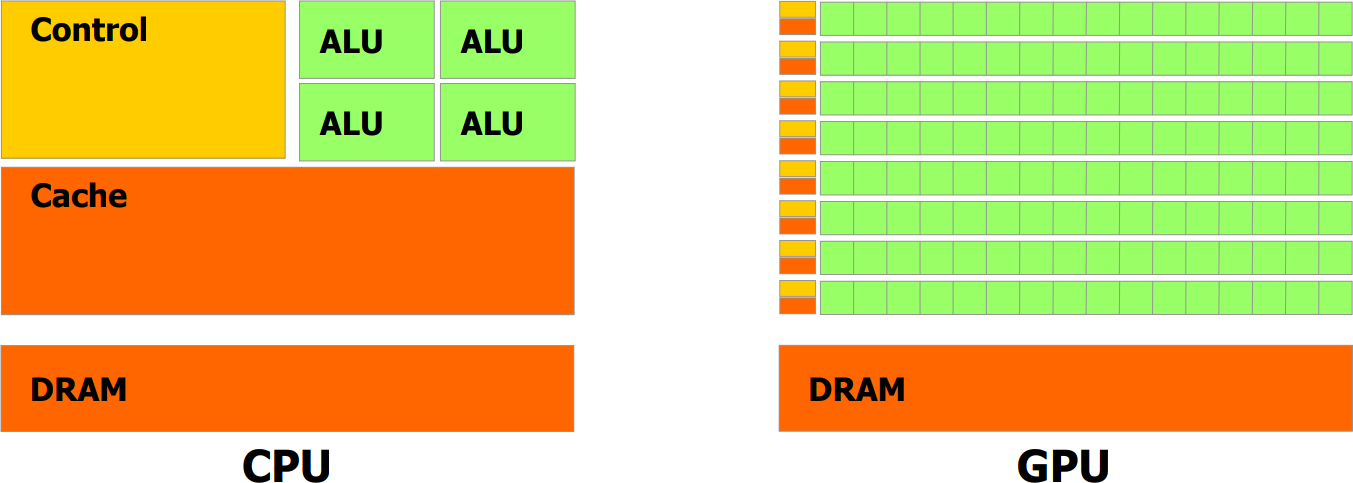
\includegraphics[width=\textwidth]{Architecture}
  \caption{\label{fig:arch} Architecture Comparison. Diagram from \cite[p3]{guide}}
\end{figure}

\par
This structure allows GPUs to excel at performing parallel tasks requiring the same operations to be performed on large sets of data, and therefore well suited to the needs of OP2, where a particular function often need to be applied to all edges, cells, or nodes in a given mesh.

\subsubsection{GPU Parallelism}
Workloads executed on a GPU are divided among a Grid of Blocks, where each Block contains a number of Threads, all executing simultaneously in parallel. To allow for easier mapping from the problem space to a Thread Identifier, the Block ID and Thread Identifiers within each block can be 1D, 2D or 3D \cite[p9]{guide}. Figure \ref{fig:threadgrid} shows an example where 2D identifiers are used.

\begin{figure}[h!]
  \centering
  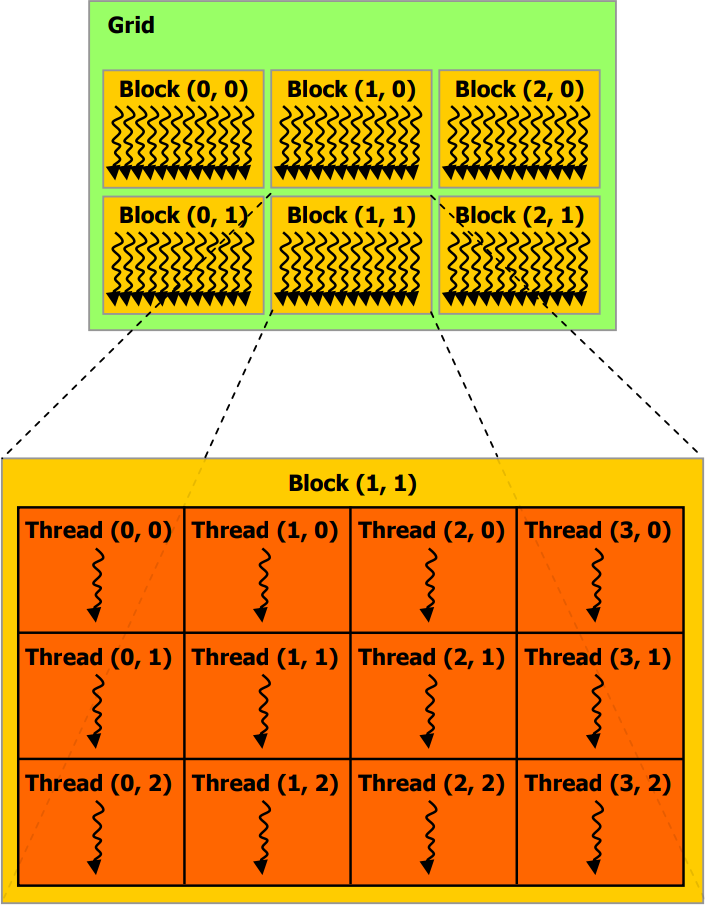
\includegraphics[width=0.6\textwidth]{threadgrid}
  \caption{\label{fig:threadgrid} 2D grid of Blocks and Threads. Diagram from \cite[p9]{guide}}
\end{figure}

\subsubsection{Programming Interface}
The CUDA C API provides two function type quantifiers that will need to be used in the generated code:
\begin{itemize}
\vspace{-.5cm}
\setlength{\itemsep}{0pt}%
\setlength{\parskip}{0pt}%
\item{\verb|__device__|}
\item{\verb|__global__|}
\vspace{-.5cm}
\end{itemize}
Both indicate that the function should be compiled to \textit{PTX}, the CUDA instruction set architecture \cite[p15]{guide}, and executed on an NVidia GPU device. The difference however, is that a function declared \verb|__global__| can be invoked from host (CPU) code, or device (GPU) code; whereas a \verb|__device__| function can only be called from code that is already executing on the device \cite[p81]{guide}.
\par
Global functions therefore act as a sort of entry point into device code. They are called using additional syntax added by the CUDA language, which allows the user to specify special paramemters for the required number of blocks, and threads per block:
\codeline{function<<< num_blocks, threads_per_block >>>( [arguments...] )}{}
\noindent Where the data type of \verb|num_blocks| and \verb|threads_per_block| can a normal C language \verb|int| type (1D), or use a CUDA type \verb|dim3| \cite[p9]{guide} to specify up to 3 dimensions. Any value left unspecified is initialised as 1 \cite[p87]{guide}. The function body will then be executed $\verb|num_blocks| \times \verb|threads_per_block|$ times, with all threads beginning at the same time. The number of threads has an upper limit depending on the hardware, for example the Kepler Architecture can support 2048 total threads per multiprocessor \cite{kepler}, for example 8 blocks of 16 $\times$ 16 threads (2 dimensions of thread IDs).
\par
Inside the function body built in variables \verb|threadIdx.x|, \verb|blockIdx.x|, and \verb|blockDim.x| can be used to determine the work which a certain thread should carry out, usually by calculating an array index from their values. Appendix \ref{app:cudaEx} is a CUDA program written during research to build familiarity with writing CUDA code, which utilises these constructs and ideas.
\par
In the next section, the OP2 Framework and it's exisiting code generation will be discussed. It can produce optimised code executable on a GPU from unoptimised sequential code, and parts of this code generator will aid in development of the new code generation script being produced for this report, with the Just-In-Time Compilation functionality as an addition.

\subsection{OP2}

\subsubsection{Exisiting Work}

This project is focussed on a contribution made to the OP2 open source library. There is a large quantity of literature available on the OP2 website \cite{op-dsl}, but the following section aims to provide enough understanding for someone unfamilar with OP2 to follow the rest of this report.
\par
OP2 is an "active library" framework \cite{op2main}, which takes a single application code written using the OP2 Application Programming Interface (API), embedded in either C or Fortran and uses source-to-source translation to produce multiple different source codes, each targetting a different optimised parallel implementation. The generated source code is then compiled, and linked against the OP2 library files to produce an executable for the original application which will run on the desired platform. It is the extra step of code generation that makes OP2 an "active" library, compared to conventional software libraries.
\par
Since this project is focused on the GPU back-end, the journal article \textit{Designing OP2 for GPU architectures} \cite{gpudesign} is necessary background material, as it covers a lot of important details from the implementation exisiting GPU framework.

\tinytitle{Designing OP2 for GPU architectures}
This article, originally published in the Journal of Parallel and Distributed Computing in 2013, describes the key design features of the current OP2 library for generating efficient code targeting GPUs based on NVidia’s \textit{Fermi} architecture. It is worth noting that \textit{Fermi} is no longer the latest architecture, and the code generation process has been modified since publication, however the article still provides useful information.
\par
One of the key points made in the paper is on the managing of data dependencies (p1454), where an operation relies on another being complete before it can begin, otherwise the result may be incorrect. Solutions include: an owner of node data which performs the computation; colouring of edges such that no two edges of the same colour update the same node; and atomic operations which perform a read-modify-write operation as a single, uninterruptable action on a 32-bit or 64-bit word residing in global or shared memory \cite[p96]{guide}. This means that a thread cannot alter the value in memory between the read and write operations of another thread, which could cause a data dependency to be violated, as all three operation are performed as a single atomic action, and therefore they cannot overlap. \\In the implementation for this project, atomic operations were selected as the best solution for this issue.
\par
The paper also introduces the consideration of data layout in memory. Figure \ref{fig:soa_v_aos} demonstrates the different layouts possible when there are multiple components for each element, in this case 4 elements with 4 components each. While using Array of Structs is the default layout, and the easier to implement, the paper concludes that transforming application code to utilise the struct-of-arrays layout is effective for reducing the total amount data transferred to and from GPU global memory, in some cases by over 50\%.


\begin{figure}[h]
  \centering
  \subfloat[Array of Structs (AOS) layout]
  {
    \begin{tikzpicture}[cell/.style={rectangle,draw=black}, ampersand replacement=\&, space/.style={minimum height=1.5em,matrix of nodes,row sep=-\pgflinewidth,column sep=-\pgflinewidth,column 1/.style={font=\ttfamily}},text depth=0.5ex,text height=2ex,nodes in empty cells]

    \matrix (A) [matrix of nodes, nodes={draw, minimum size=8mm}]{
        0 \& 1 \& 2 \& 3 \& 0 \& 1 \& 2 \& 3 \& 0 \& 1 \& 2 \& 3 \& 0 \& 1 \& 2 \& 3\\};
    \end{tikzpicture}
  }

  \quad

  \subfloat[Struct of Arrays (SOA) layout]
  {
    \begin{tikzpicture}[cell/.style={rectangle,draw=black}, ampersand replacement=\&, space/.style={minimum height=1.5em,matrix of nodes,row sep=-\pgflinewidth,column sep=-\pgflinewidth,column 1/.style={font=\ttfamily}},text depth=0.5ex,text height=2ex,nodes in empty cells]

    \matrix (A) [matrix of nodes, nodes={draw, minimum size=8mm}]{
      0 \& 0 \& 0 \& 0 \& 1 \& 1 \& 1 \& 1 \& 2 \& 2 \& 2 \& 2 \& 3 \& 3 \& 3 \& 3\\};
    \end{tikzpicture}
  }
  \caption{\label{fig:soa_v_aos} Data layouts. Diagram reproduced from \cite{gpudesign}}
\end{figure}

\noindent The SoA layout is enabled by setting the value of an environment variable: \verb|OP AUTO SOA=1| prior to code generation \cite[p13]{manual}. In the Implementation section (Section \ref{s:impl}) the differences in generated code when this is enabled will be explained in greater detail.
\par
The existing solution is able to generate optimised CUDA code for a parallel loop where the resulting code can map set elements to a GPU thread it will be processed by, therefore operating on many set elements at once in parallel. It is important to note that the existing implementation for CUDA code generation produces a solution that is compiled entirely ahead of time, i.e.\ prior to the inputs being known, and therefore is not able to make optimisations based on the mesh input. This project aims to bridge this gap, and determine if there is benefit to be gained from such optimisations.
\par
Since OP2 enforces that the order in which the function is applied to the members of the set must not affect the final result \cite[p4]{manual}, the consideration for not violating data dependencies between iterations is removed in the generated code, and therefore loop iterations can be scheduled in any order, based on best performance.

\subsubsection{OP2 Applications}
There are a number of industrial applications that have been implemented using the OP2 active library framework, which would immediately benefit from further optimisation of the generated code, including: Airfoil \cite{airfoil} - a non-linear 2D inviscid airfoil code; Hydra \cite{hydra} - Rolls Royce’s turbomachinery simulator; and Volna \cite{volna} - a finite-volume nonlinear shallow-water equation solver used to simulate tsunamis.
\par
They make use of the abstraction provided by the OP2 API to allow scientists and engineers to focus on the description of the problem, and separates the consideration for parallelism, data-movements, and performance into the OP2 library and code generation.
\par
A further benefit is that such applications can be ported onto a new generation of hardware, which could be developed in the future. Only the OP2 backend library would need to be modified to provide support the new hardware, instead of every application individually. This portability can save both time and money in development of HPC applications if multiple different hardware platforms are desired to be used.
\par
Later in this report we will see Airfoil used for benchmarking runtime, to determine whether the new optimisation presented in the report is likely to provide benefit to other OP2 applications.

\subsubsection{OP2 Results}
The optimisation of the Hydra turbomachinery simulator was presented in a 2016 paper titled \textit{Acceleration of a Full-scale Industrial CFD Application with OP2} \cite{hydrapaper}. This paper compares the newer OP2 framework with it's predecessor OPS \cite{ops}, as well as benchmarking the application against OP2 code generated utilising OpenMP \cite{OpenMP} and MPI \cite{MPI} for thread and process level parallelism respectively. Initially, OP2's GPU code generation was outperformed by both OPS generating MPI, and most of the OP2 MPI implementations - completing 45\% slower than the best CPU performance (2 CPUs, 24 MPI processes).
\par However, after some parameters had been tweaked including modifying the block sizes and enabling the Struct-Of-Arrays data layout, a single K20 GPU was able to achieve nearly $1.8\times$ speedup over the original OPlus version, and close to $1.5\times$ over the MPI version of Hydra with OP2. It is worth noting that these MPI implementations are already optimised parallel versions, not sequential implementations, so a speedup of 150\% is a very significant result.
\clearpage

\subsection{Just-In-Time Compilation}
\label{ss:rw_JIT}

The term "Just-In-Time Compilation" is most commonly associated with the Java programming language, and particularly the Java Run-time Environment (JRE), as "JIT" Compilation is an integral part of the design and usage of the Java Virtual Machine (JVM).

\par The Java compiler (\verb|javac|) compiles code into platform independant "bytecode" \cite{javac}, then at run-time this bytecode can be interpretted, or compiled a second time by the JVM into native code, and optimised specifically for the machine it is running on. It can also take the program's inputs into account, since they will be known and fixed at run-time.
\par
This re-compilation from bytecode to native code is only done for "hot" sections which are dominating the runtime \cite{javac}, while the rest continues to be interpretted, as it is not worth the time cost to recompile. Chapter 4 of \textit{Java Performance: The Definitive Guide} \cite{javaPerf} contains further detail on the JIT compiler and its impact on the performance of Java.
\par
The core idea of recompiling code at run-time to obtain performance is the inspiration for the new optimisation investigated in this report, and the origin of its name. However, the Java approach does not exactly map onto OP2. In the existing framework, there is no possibility of intermediate code, and no Virtual Machine in which the binary will execute that can profile the running code and react to "hot sections. Instead, an alternative source file at the same "level" above native code is created (see Figure \ref{fig:jit_compare}). This new source code that has been translated will be able to utilise assertions made using the input data, and so is compiled and used in place of the equivalent but unoptimsed functions compiled ahead of time. The design of the JIT compilation system for OP2 will be covered in greater detail in Section \ref{s:spec}.

\begin{figure}[h!]
  \vspace{2em}
  \makebox[\textwidth][c]{
  \resizebox{1.1\textwidth}{!}{
\begin{tikzpicture}

    \tikzstyle{arr} = [->, >=stealth, line width=1mm];
    \tikzstyle{rowtitle} = [text width=7em, text centered, font=\bfseries];

    %\draw [help lines] (0,0) grid (10,6);

    \node [rowtitle] at (0,4) (source) {Source Code};
    \node [rowtitle] at (0,2) (inter) {Intermediate Representation};
    \node [rowtitle] at (0,0) (native) {Native Instructions};

    \draw [loosely dashed] (-1.5,1) -- (17.5,1);
    \draw [loosely dashed] (-1.5,3) -- (17.5,3);

    \draw (2,-1) -- (2,6);
    \draw (9,-1) -- (9,6);
    \draw (17,-1) -- (17,6);

    \node [anchor=north] at (5.5,6) (JAVA) {\textbf{JAVA}};

    \node [wblock] at (3.5,4) (jsource) {Java Source};
    \node [wblock] at (5.5,2) (jbyte) {Java ByteCode};
    \node [wblock] at (7.5,0) (jsvm) {Execution in JVM};

     \node [anchor=north] at (13,6) (OP2) {\textbf{OP2}};
    %
     \node [wblock] at (10.5,4) (appsource) {Application Source};
     \node [wblock] at (13,4) (tsource) {Translated Source};
     \node [wblock] at (15.5,0) (bin) {Native Binary};

     \draw [arr] (appsource.north) to [out=30,in=150] (tsource.north);
     \draw [arr] (tsource.east) to [out=-30,in=90] (bin.north);

     \draw [arr] (jsource.east) to [out=0,in=90] (jbyte.north);
     \draw [arr] (jbyte.east) to [out=0,in=90] (jsvm.north);

\end{tikzpicture}
  }}

  \caption{Comparison of Java and OP2 JIT}
  \label{fig:jit_compare}
\end{figure}

\subsubsection{Related Work}

While Java's JIT compilation gives a good indication that there is real benefit to be gained from using the technique, it's implementation doesn't translate well on to the active library workflow. While researching more similar applications of the concept, the \textit{easy::JIT} library was discovered.\\
\hspace{\parindent}\tinytitle{easy::JIT} \textit{easy::JIT} \cite{eJIT} is a library created by Juan Manuel Martinez Caamaño and Serge Guelton of \textit{Quarkslab} \cite{Quarkslab}. It targets C++ code, and utilises \verb|clang| \cite{clang} as the compiler, which is built using the Low Level Virtual Machine (LLVM) framwork. It therefore can make use of the LLVM's Intermediate Representation, where other C compilers like \verb|gcc| cannot. \textit{easy::JIT} does also differ from this project however, as it utilises code generation at run-time, and a cache of code to ensure this does not need to be done on every execution. The OP2 implementation discussed in this report will generated all of the code ahead of time, as this is a slow process.
\par
Applications developed for OP2 are not currently limited to only LLVM-based C compilers like \verb|clang|, although a translator using LLVM Intermediate Representation to replace the current Python and MatLab source-to-source translation scripts is currently in development \cite{op2clang}. This would bring it more in line with Java, having an original source, an intermediate representation, and then native code after the second compilation stage.\\
The implementation completed for this report is building on the compiler agnostic OP2 implementation, and therefore will not utilise LLVM .
